% FlightLog Black Box: CA3 project report.
% Build: pdflatex report.tex (twice, for the table of contents), or upload this folder with ../figures to Overleaf.
\documentclass[11pt,a4paper]{article}

\usepackage[T1]{fontenc}
\usepackage[utf8]{inputenc}
\usepackage{lmodern}
\usepackage[margin=2.3cm]{geometry}
\usepackage{graphicx}
\usepackage{booktabs}
\usepackage{tabularx}
\usepackage{array}
\usepackage[table]{xcolor}
\usepackage{caption}
\usepackage{float}
\usepackage{enumitem}
\usepackage{amsmath}
\usepackage{listings}
\usepackage{parskip}
\usepackage[hidelinks]{hyperref}

\graphicspath{{figures/}{../figures/}}
\definecolor{orange}{HTML}{F26B1D}
\definecolor{ink}{HTML}{1B1F2A}
\definecolor{muted}{HTML}{5B6577}
\captionsetup{font=small,labelfont=bf}
\setlist{itemsep=2pt,topsep=4pt}
\newcolumntype{L}{>{\raggedright\arraybackslash}X}
\renewcommand{\arraystretch}{1.25}
\newcommand{\code}[1]{\texttt{\detokenize{#1}}}
\lstset{basicstyle=\ttfamily\small,columns=fullflexible,frame=single,rulecolor=\color{muted!40},
        breaklines=true,keepspaces=true}

\begin{document}

% ------------------------------------------------------------------ title page
\begin{titlepage}
  \centering
  \vspace*{2.5cm}
  {\color{orange}\large\bfseries CA3 \quad Software Automation Lab \quad Project 29\par}
  \vspace{1.2cm}
  {\Huge\bfseries\color{ink} FlightLog Black Box\par}
  \vspace{0.6cm}
  {\Large Automated health checks for ArduPilot drone flight logs\par}
  \vspace{2.2cm}
  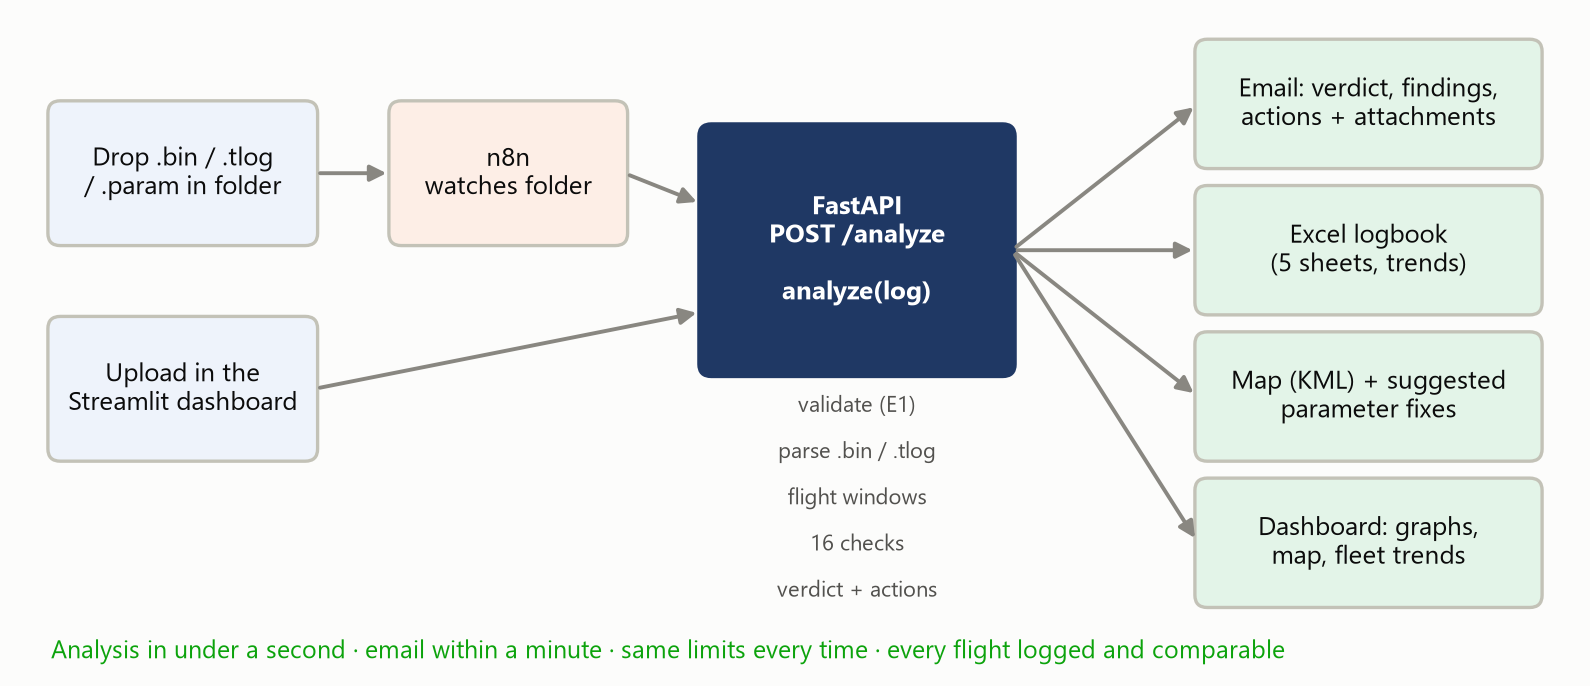
\includegraphics[width=0.95\textwidth]{workflow_proposed.png}\par
  \vspace{2.2cm}
  {\large Aarushi Rudra \quad Zahra Modi \quad Harsh Narain\par}
  \vfill
  {\large October 2026\par}
\end{titlepage}

\begin{abstract}
After every test flight of our ArduPilot quadcopter, someone used to open the flight log in Mission Planner
or UAV Log Viewer and judge vibration, battery, estimator and motor graphs by eye. The check was slow,
depended on the reviewer, and left no record that allowed flights to be compared. FlightLog Black Box
automates the whole review. A log dropped into a folder (or uploaded in a web dashboard) is validated,
parsed and split into flight phases, then 16 health checks run against limits kept in one configuration
file. The result is a Healthy, Warning or Critical verdict, the reasons, recommended actions and suggested
parameter fixes, delivered by email together with an Excel logbook of every flight. The workflow is
orchestrated with n8n, the analysis runs as a FastAPI service in Python, and a Streamlit dashboard shows
single flights and fleet trends. Seven exception cases are handled and 88 automated tests cover the
scenarios of the test plan. On the team's 28 real log files the system analysed six flight logs and found
real faults in all of them, most importantly a battery that collapsed under load and caused thrust loss on
24 September, with a low-battery failsafe set too low ever to trigger.
\end{abstract}

\tableofcontents
\newpage

% ------------------------------------------------------------------ 1
\section{Introduction}

\subsection{Problem statement}
ArduPilot flight controllers record a DataFlash log (\code{.bin}) on their SD card during every flight, and the
ground station can save the telemetry stream as a \code{.tlog}. These logs hold everything needed to judge
whether the drone is healthy: vibration levels, battery voltage and current, how well the position estimator
agrees with the sensors, motor outputs, and every error the firmware raised.

In our team, reviewing a log meant opening it in Mission Planner or UAV Log Viewer and clicking through graphs.
That review is slow, it depends on who does it and which graphs they remember to open, there are no fixed
limits, and nothing is recorded per flight. Problems that build up across flights, such as rising vibration
from a loosening propeller or an ageing battery, go unnoticed until something fails. Drone fleet operators
and maintenance teams face the same problem at a larger scale.

\subsection{Objectives}
\begin{itemize}
  \item Turn any ArduPilot flight log into a Healthy / Warning / Critical verdict with reasons, without anyone
        opening a graph.
  \item Use fixed, documented limits kept in one file, so every flight is judged the same way.
  \item Keep a record of every flight in an Excel logbook and compare each flight with the same drone's earlier
        flights.
  \item Run hands-free: dropping a log in a folder is enough, and the team is told by email.
  \item Handle bad input (wrong files, corrupt logs, duplicates, bench logs) without breaking or going silent.
\end{itemize}

\subsection{Scope}
In scope: ArduPilot DataFlash \code{.bin} and MAVLink \code{.tlog} logs, parameter files for a pre-flight check,
16 automated checks, the Excel logbook, email, the Streamlit dashboard and the n8n workflow. Out of scope:
live telemetry, PX4 \code{.ulg} logs, ROS~2 bag files, and repairing the drone.

% ------------------------------------------------------------------ 2
\section{Existing process}

Figure~\ref{fig:existing} shows the manual review as it was done before this project.

\begin{figure}[H]
  \centering
  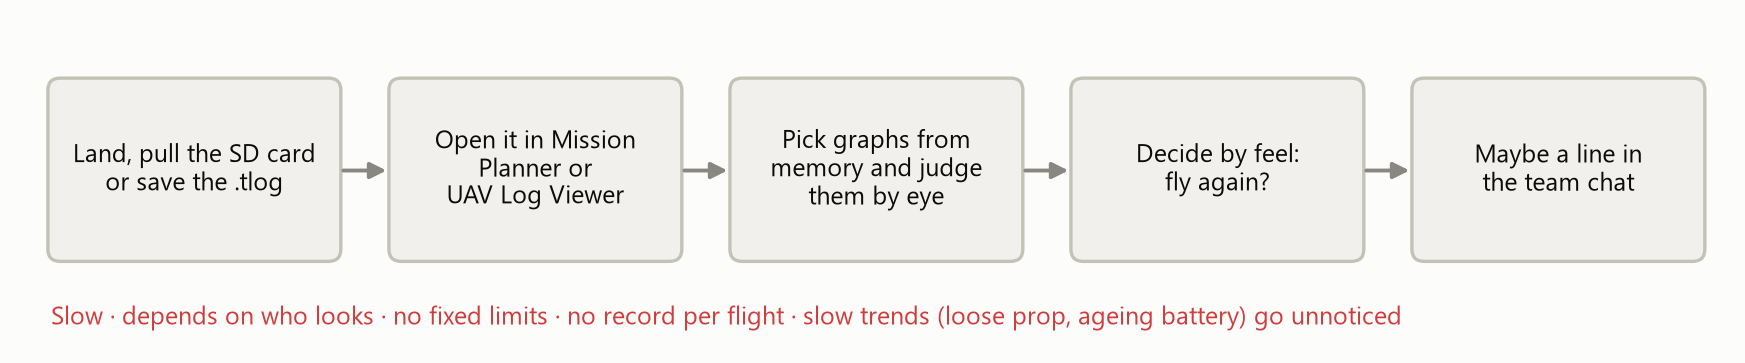
\includegraphics[width=\textwidth]{workflow_existing.png}
  \caption{The manual log review. Every decision depends on one person's judgement.}
  \label{fig:existing}
\end{figure}

\begin{enumerate}
  \item Land, then pull the log from the SD card or save the telemetry log.
  \item Copy it to someone's laptop under whatever file name they choose.
  \item Open it in Mission Planner or UAV Log Viewer.
  \item Choose which graphs to open (\code{VIBE}, \code{BAT}, \code{CTUN}, \code{XKF4}, \ldots) from memory.
  \item Judge ``looks fine'' by eye, with no fixed thresholds.
  \item Perhaps post a line in the team chat. Nothing is recorded per flight.
  \item Slow trends across flights go unnoticed.
\end{enumerate}

\textbf{Pain points:} slow, inconsistent between reviewers, no history, and easy to skip after a flight that
looked fine.

% ------------------------------------------------------------------ 3
\section{Proposed automated workflow}

The automation replaces every step of the manual review; a person steps in only when a flight is flagged
(Figure~\ref{fig:proposed}). There are two ways in: drop a file into a watched folder, where n8n picks it up,
or upload it in the Streamlit dashboard. Both call the same FastAPI endpoint, which runs one Python function,
\code{analyze(log_path)}. Its result drives four outputs: the email, the Excel logbook, a KML flight map with
suggested parameter fixes, and the dashboard.

\begin{figure}[H]
  \centering
  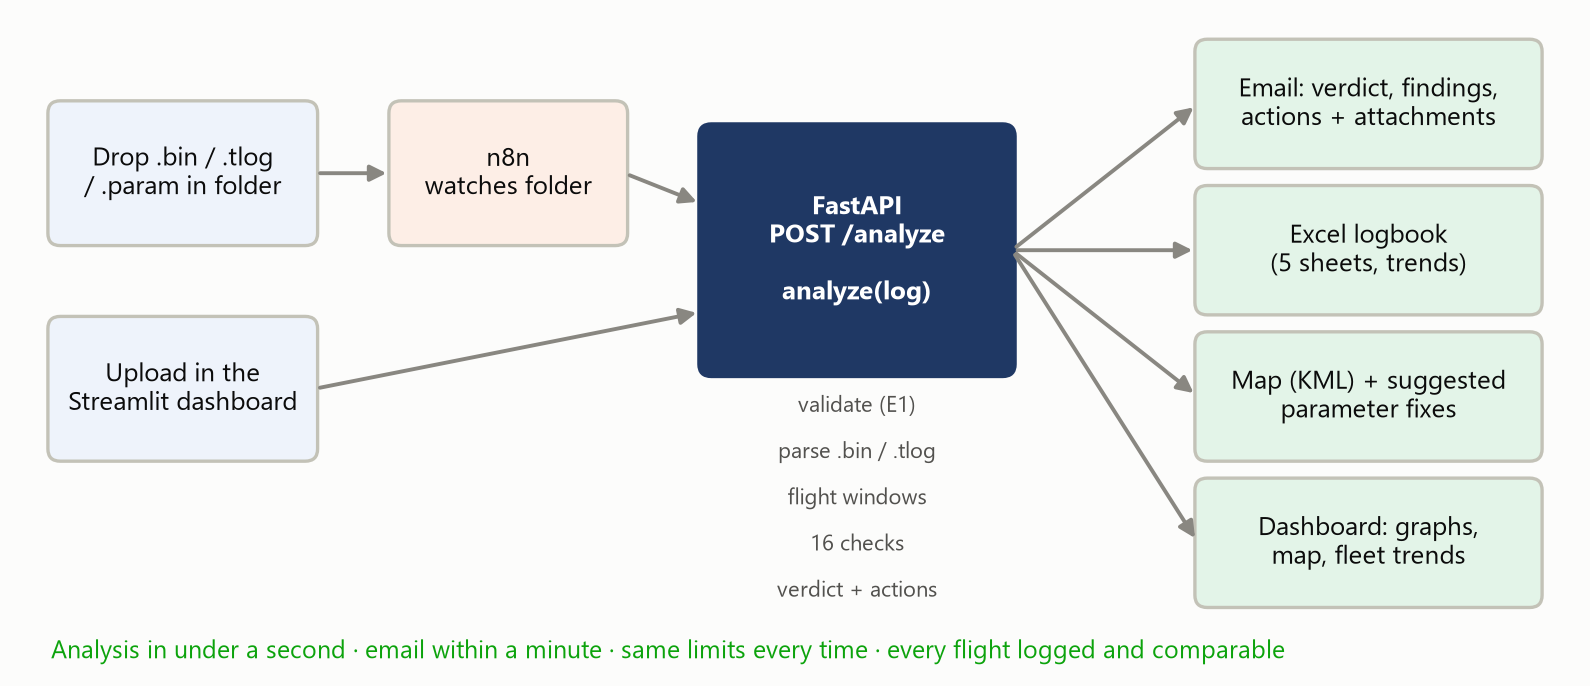
\includegraphics[width=\textwidth]{workflow_proposed.png}
  \caption{The automated workflow. Both entry points call the same analysis, so they always agree.}
  \label{fig:proposed}
\end{figure}

A valid log gets the full report. A file that fails validation (not a log, corrupt, never armed) is still
recorded in the logbook's Exceptions sheet, and the team is still emailed, so nothing disappears silently.

% ------------------------------------------------------------------ 4
\section{Architecture and technology}

\begin{table}[H]
  \centering
  \begin{tabularx}{\textwidth}{@{}p{3.3cm}p{4.2cm}L@{}}
    \toprule
    \textbf{Layer} & \textbf{Tool} & \textbf{Job} \\
    \midrule
    Trigger and delivery & n8n 2.43, self-hosted with \code{npx} & Watch the folder, read the file, post it to the API, email the team
      (SMTP with a Gmail App Password) \\
    API & FastAPI and uvicorn & \code{POST /analyze}, \code{GET /files/...}, \code{/logbook}, \code{/ledger}, \code{/health} \\
    Core & Python 3.11, pymavlink, pandas, numpy & Validate, parse, flight windows, 16 checks, verdict, actions \\
    Configuration & \code{thresholds.yaml} & Every limit in one file, so tuning needs no code change \\
    Outputs & openpyxl, HTML email, KML & Excel logbook, email body, flight map, Mission Planner \code{.param} fixes \\
    Web front end & Streamlit & Upload a log, verdict card, graphs, map, fleet logbook \\
    Tests & pytest & 88 tests: the ten scenarios of the test plan and the parts around them \\
    \bottomrule
  \end{tabularx}
  \caption{Technology stack.}
\end{table}

UiPath was not used. Parsing binary flight logs and running numerical checks needs Python libraries, and n8n
does the orchestration an RPA bot would do. The repository layout is:

\begin{lstlisting}
flightlog-blackbox/
  blackbox/       validate, parse (.bin), tlog (.tlog), windows, checks, verdict, advice,
                  pipeline (analyze), preflight, history, exports, report, logbook
  api.py          FastAPI service       app.py      Streamlit dashboard
  n8n/            workflow JSON         scripts/    setup_n8n.py, start.ps1
  thresholds.yaml every limit           tests/      88 pytest tests and a synthetic log writer
\end{lstlisting}

% ------------------------------------------------------------------ 5
\section{Implementation}

\subsection{Validation by content}
The file type is decided from its bytes, not its name, so a photo renamed to \code{.bin} is rejected and a
real log saved under a temporary name without an extension is still read.

\begin{itemize}
  \item \textbf{DataFlash (\code{.bin}):} every record starts with \code{0xA3 0x95}, and the first is the format
        record \code{0x80}.
  \item \textbf{Telemetry (\code{.tlog}):} an 8-byte big-endian receive time in microseconds (a plausible date)
        followed by a MAVLink frame starting with \code{0xFE} or \code{0xFD}.
  \item \textbf{Raw link capture (\code{.rlog}):} five back-to-back MAVLink frames of one version somewhere in the
        first 4~KB. These have no timestamps, so they are rejected with a message naming the file to upload instead.
  \item \textbf{Parameter file:} plain-text \code{NAME,VALUE} lines (Mission Planner) or the QGroundControl format,
        which triggers the pre-flight check instead of a flight analysis.
\end{itemize}

\subsection{Parsing}
\code{.bin} logs are read with pymavlink's \code{DFReader_binary} directly. The generic
\code{mavutil.mavlink_connection} picks its reader from the file extension and would misread an upload saved
under a temporary name. Each message type becomes a pandas DataFrame with a time column in seconds. If the
parser stops at a corrupt record, everything read so far is kept and the log is marked incomplete (E2).

A \code{.tlog} is mapped onto the same tables, so the checks do not care where the data came from
(Table~\ref{tab:tlog}). Telemetry arrives at only 2--4~Hz, so the report notes that it has reduced detail.

\begin{table}[H]
  \centering
  \begin{tabularx}{\textwidth}{@{}p{2.6cm}L@{}}
    \toprule
    \textbf{Table} & \textbf{Built from MAVLink messages} \\
    \midrule
    \code{VIBE} & \code{VIBRATION} (one value per axis, a clip counter per accelerometer) \\
    \code{BAT}, \code{POWR} & \code{SYS_STATUS}, \code{POWER_STATUS} \\
    \code{CTUN} & \code{VFR_HUD} throttle, \code{GLOBAL_POSITION_INT} altitude, \code{NAV_CONTROLLER_OUTPUT} target \\
    \code{ATT} & \code{ATTITUDE} with desired angles from \code{NAV_CONTROLLER_OUTPUT} \\
    \code{XKF4}, \code{RCOU} & \code{EKF_STATUS_REPORT}, \code{SERVO_OUTPUT_RAW} \\
    \code{ARM}, \code{MODE} & \code{HEARTBEAT} (armed flag, custom mode) \\
    \code{ERR}, \code{MSG} & \code{STATUSTEXT}, with known texts such as ``Potential Thrust Loss'' mapped to error codes \\
    \bottomrule
  \end{tabularx}
  \caption{How a telemetry log is mapped onto the DataFlash tables the checks use.}
  \label{tab:tlog}
\end{table}

\subsection{Flight windowing}
A log contains much more than flight: minutes on the bench powered by USB (0~V battery, a radio failsafe
because no receiver is connected), arming without taking off, and the takeoff and landing transients. Judging
the whole log would raise false alarms, so the log is first split into windows (Figure~\ref{fig:windows}):

\begin{itemize}
  \item \textbf{Armed:} from the \code{EV} armed/disarmed events or \code{ARM} records.
  \item \textbf{Airborne:} from the land detector's \code{NOT_LANDED} and \code{LAND_COMPLETE} events; logs
        without them fall back to altitude above the ground level at arming.
  \item \textbf{Trimmed:} airborne minus 3~s after takeoff and before landing.
  \item \textbf{Hover:} climb rate below 0.25~m/s and tilt below 5$^\circ$ for at least 2~s.
  \item \textbf{Altitude-controlled:} time in flight modes where the altitude target is meaningful.
\end{itemize}

Each check runs only in its window, and checks on multi-instance sensors (several IMUs, batteries or EKF cores)
are evaluated per instance, reporting the worst one, so interleaved rows from different sensors are never mixed.

\begin{figure}[H]
  \centering
  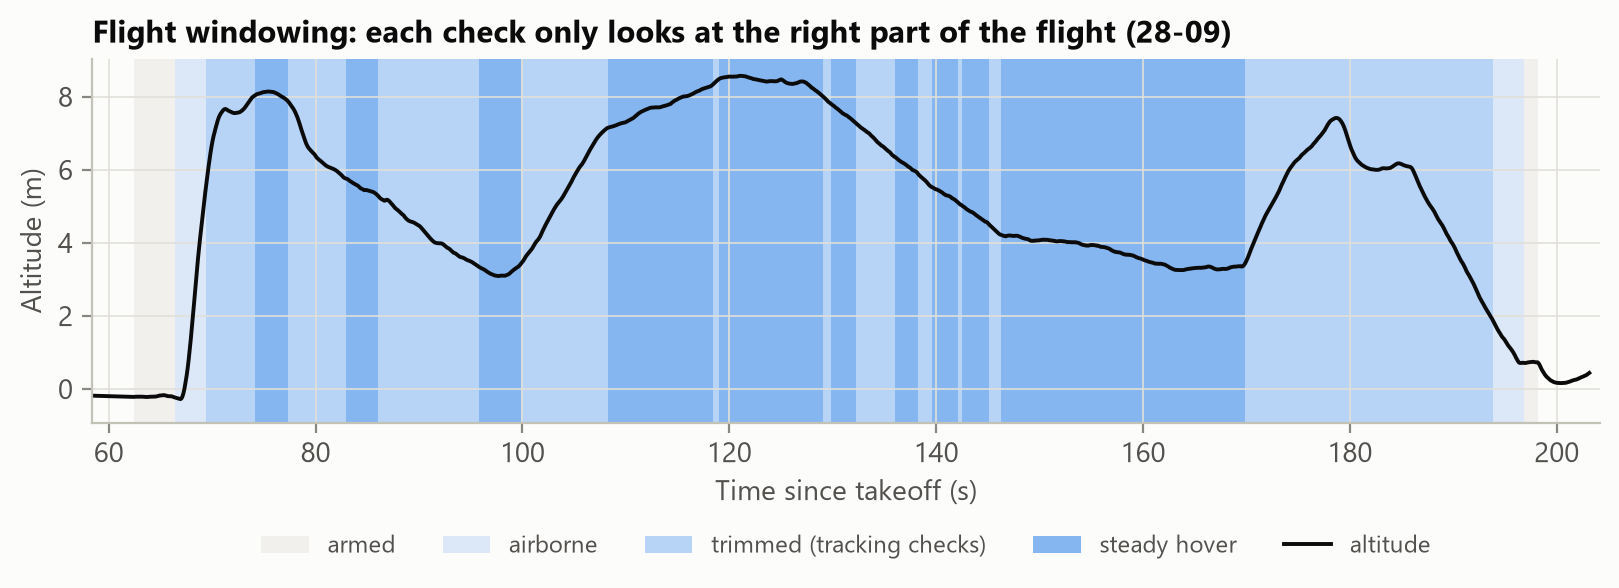
\includegraphics[width=\textwidth]{windows.png}
  \caption{Flight windows on the 28 September flight.}
  \label{fig:windows}
\end{figure}

\subsection{The 16 health checks}
Table~\ref{tab:checks} lists the checks and their limits. Vibration and EKF limits come from the ArduPilot
documentation; the others are team-set starting values, to be tuned on two or three clean flights by setting
each warning comfortably above the clean maximum. Short spikes are ignored by using a 1-second rolling median.
A check whose messages are missing from the log shows ``Not available'' with the logging option to enable (E3)
and does not change the verdict.

\begin{table}[H]
  \centering
  \small
  \begin{tabularx}{\textwidth}{@{}rp{3.6cm}Lp{3.3cm}@{}}
    \toprule
    \textbf{\#} & \textbf{Check} & \textbf{What is measured} & \textbf{Warning / Critical} \\
    \midrule
    1 & Vibration & \code{VIBE} X/Y/Z, sustained maximum & $>30$ / $>60$ m/s$^2$ \\
    2 & Accelerometer clipping & rise of the clip counter while airborne & $>0$ / $>100$ \\
    3 & Cell voltage under load & lowest sustained voltage per cell & $<3.5$ / $<3.3$ V \\
    4 & Voltage sag & resting minus loaded voltage per cell & $>0.3$ / $>0.5$ V \\
    5 & Board supply & \code{POWR.Vcc} minimum while armed & $<4.8$ / $<4.5$ V \\
    6 & Hover throttle & median throttle output in hover & $>0.60$ / $>0.75$ \\
    7 & Altitude hold & target minus actual altitude, 95th percentile & $>0.3$ / $>0.6$ m \\
    8 & Attitude tracking & commanded minus actual roll/pitch, 95th percentile & $>5^\circ$ / $>10^\circ$ \\
    9 & Estimator health & EKF innovation test ratios held for 1 s & $>0.8$ / $>1.0$ \\
    10 & Motor balance & spread of motor outputs, worst 5 s chunk & $>100$ / $>200$ $\mu$s \\
    11 & Hard landing & impact acceleration and descent rate at touchdown & 3 g, 1 m/s / 5 g, 2 m/s \\
    12 & Errors and failsafes & \code{ERR} records while armed & any / crash, EKF, thrust loss \\
    \rowcolor{orange!10} 13 & External navigation gaps & longest gap in vision data while airborne & $>0.2$ / $>0.5$ s \\
    \rowcolor{orange!10} 14 & Configuration & battery parameters against the pack actually fitted & mismatch: Warning \\
    \rowcolor{orange!10} 15 & Vibration spectrum & FFT peak of IMU batch samples against the notch filter & peak missed: Warning \\
    \rowcolor{orange!10} 16 & Compass interference & change of field strength with battery current & $>30$ / $>60$ \% \\
    \bottomrule
  \end{tabularx}
  \caption{The health checks. Shaded rows were added beyond the 12 in the project plan.}
  \label{tab:checks}
\end{table}

Some details matter for correct results:
\begin{itemize}
  \item The battery cell count is not stored in the log. It is taken from \code{MOT_BAT_VOLT_MAX} (4.2~V per cell)
        unless that disagrees with the voltage at arming, which happened in our logs: a 6S setting on a 3S pack.
  \item Hover throttle uses the actual throttle output, not the learned estimate \code{ThH}, which ArduPilot caps.
  \item The clip counter is cumulative, so only its rise inside airborne windows counts, excluding the landing impact.
  \item Motor balance takes the worst 5-second chunk instead of one average, so a motor that weakens halfway
        through a flight is not averaged away.
  \item Errors logged on the bench or after disarming are ignored; a crash check logs just before it disarms, so it
        stays inside.
\end{itemize}

\paragraph{Check 15, vibration spectrum.} The IMU batch sampler logs raw gyro samples at the full sensor rate. A
Hann-windowed FFT of each batch is averaged, the strongest peak between 20 and 450~Hz is found, and it is compared
with the harmonic notch filter's centre frequency and bandwidth (\code{INS_HNTCH_*}). If the notch is off or misses
the peak, the check suggests notch settings for the measured frequency.

\paragraph{Check 16, compass interference.} The Earth's magnetic field has the same strength whatever the drone's
attitude, so any change of the measured field strength $|B|$ with battery current $I$ comes from the power wiring.
A straight line is fitted,
\begin{equation}
  |B| \approx B_0 + k\,I, \qquad \text{interference} = \frac{|k|\, I_{\max}}{B_0} \times 100\,\%,
\end{equation}
and graded with ArduPilot's compass--motor calibration guidance: under 30\% is acceptable, over 60\% is unusable.

\subsection{Verdict and recommended actions}
Any Critical makes the flight Critical, any Warning makes it Warning, otherwise it is Healthy. ``Not available''
is ignored. The recommended actions are plain rules on the check results, most specific first. Linked causes
come first, so the team fixes one cause instead of three symptoms: a battery whose voltage collapsed together
with a thrust-loss error produces ``ground this battery'', covering the voltage, sag, error and hard-landing
findings in one action. Check 10 names the motor output that works hardest, and check 12 turns error codes into
plain language (``Potential thrust loss'' instead of \code{THRUST_LOSS_CHECK/1}).

\subsection{Outputs}
\begin{itemize}
  \item \textbf{Email} (Figure~\ref{fig:email}): verdict banner, findings with measured value, limit and time,
        recommended actions, comparison with earlier flights, and notes. It is sent as HTML with a plain-text
        alternative.
  \item \textbf{\code{suggested_fixes.param}:} corrected parameter values in Mission Planner's format, each with
        the reason, to review and load.
  \item \textbf{\code{flight_path.kml}:} the GPS track for Google Earth, coloured by verdict, with each finding
        pinned where it happened.
  \item \textbf{Excel logbook} (Figure~\ref{fig:logbook}): sheets Flights, Findings, Exceptions, Pre-flight and
        Trends (four line charts). It is rebuilt from a JSON-lines record on every save, because openpyxl drops
        existing charts when it edits a workbook.
  \item \textbf{Pre-flight GO / NO-GO:} a parameter file dropped into the folder is checked for a battery failsafe
        that cannot fire, a missing battery monitor, radio failsafe off, pre-arm checks off, missing logging and
        notch-filter settings.
\end{itemize}

\begin{figure}[H]
  \centering
  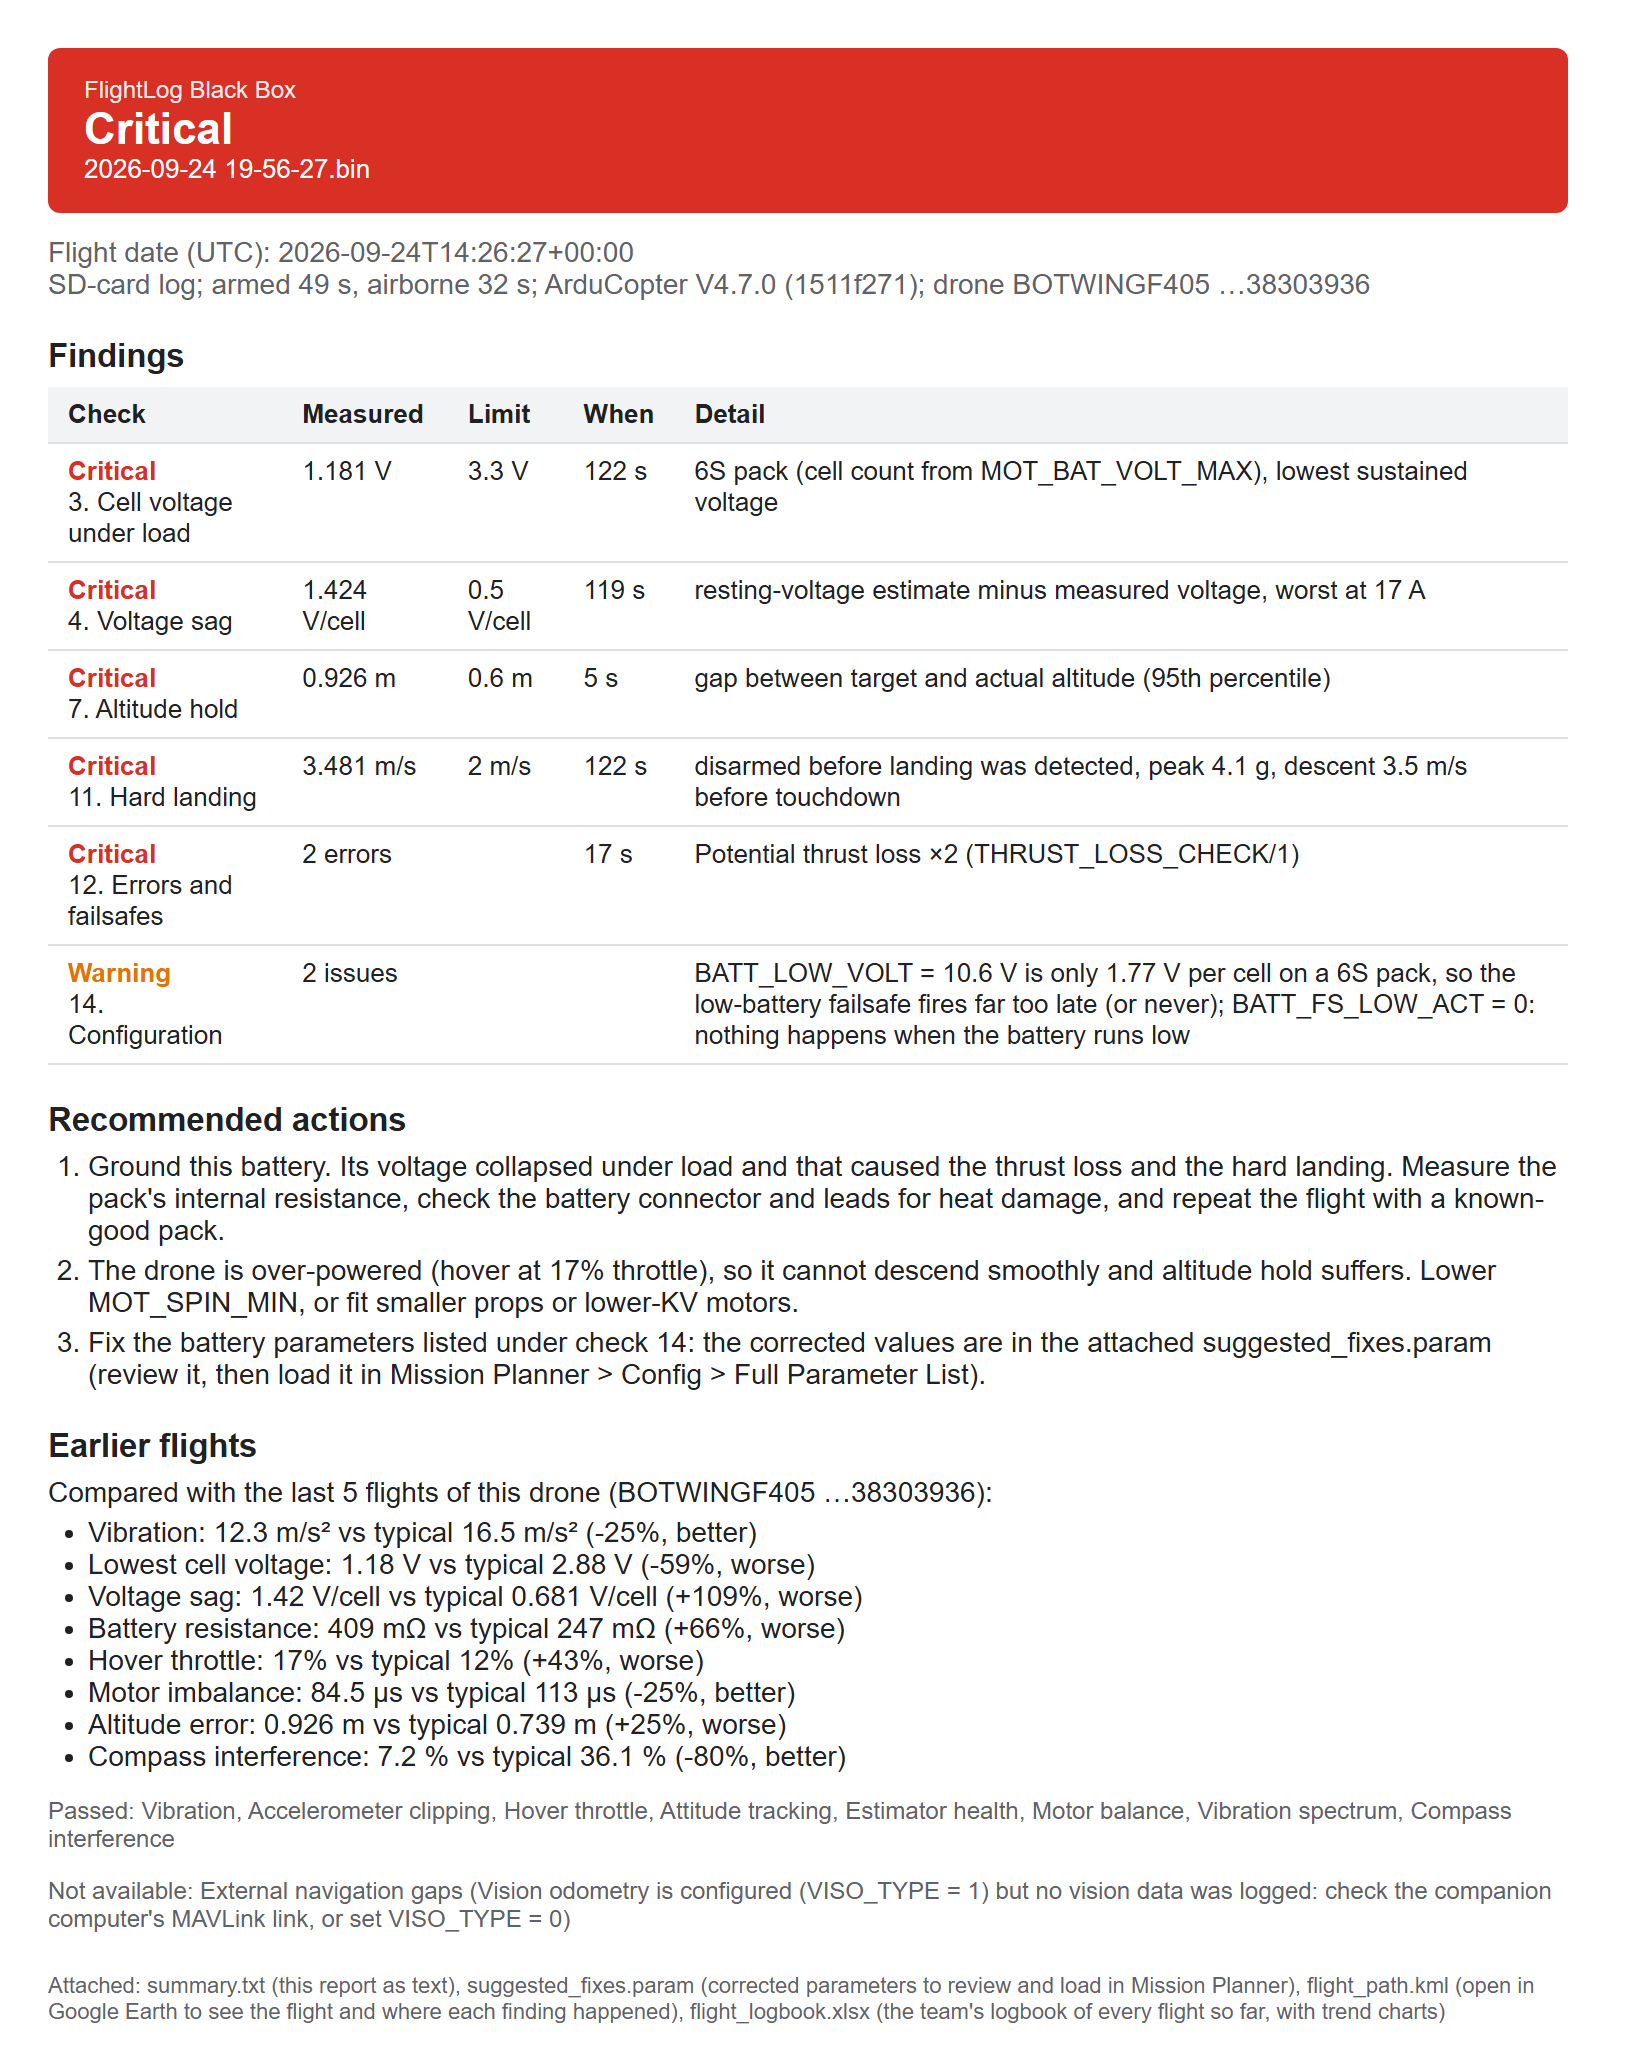
\includegraphics[width=0.62\textwidth]{email.png}
  \caption{The email for the 24 September flight.}
  \label{fig:email}
\end{figure}

\begin{figure}[H]
  \centering
  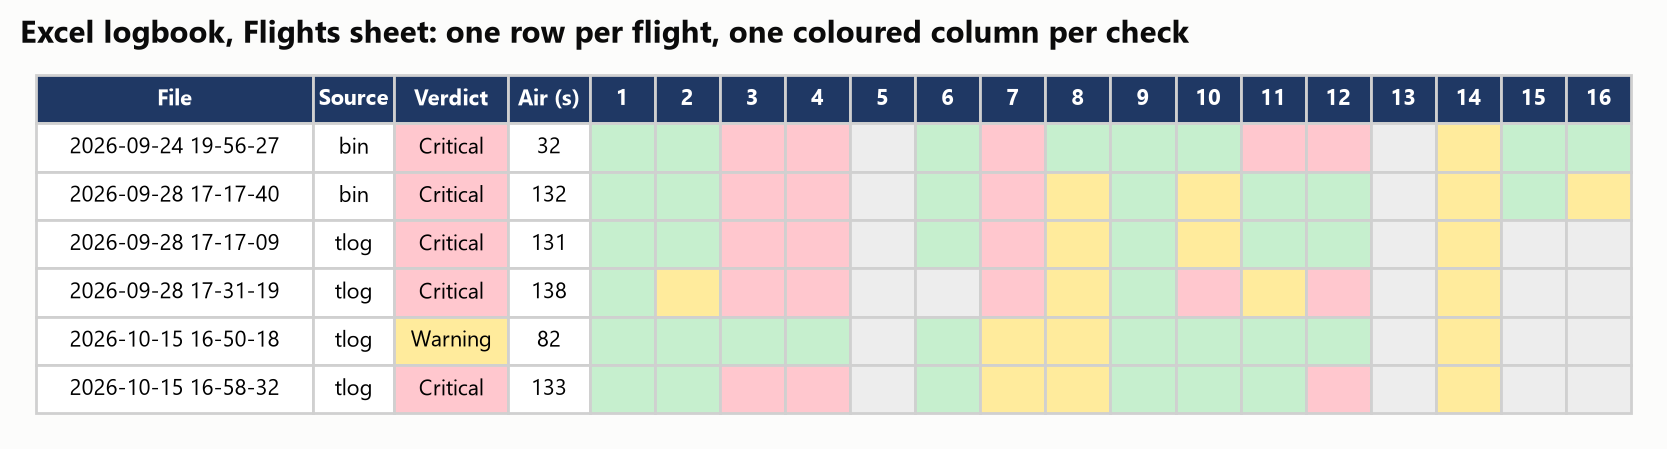
\includegraphics[width=\textwidth]{logbook_flights.png}
  \caption{The Flights sheet of the Excel logbook after the six real flight logs.}
  \label{fig:logbook}
\end{figure}

\subsection{History and tamper-evident ledger}
Each flight is compared with the same drone's last five flights. The drone is recognised by the flight
controller's board name and CPU serial number, which the firmware prints at boot, so this works across
\code{.bin} and \code{.tlog} files without labelling. A metric that changed by more than 20\% from its typical
value is reported as better or worse.

Every processed file is entered in a ledger keyed by its SHA-256 hash. Each entry stores a hash over the previous
entry's hash and its own fields,
\begin{equation}
  h_i = \mathrm{SHA256}\left(h_{i-1} \,\|\, \text{file hash} \,\|\, \text{date} \,\|\, \text{name} \,\|\,
        \text{status} \,\|\, \text{verdict}\right), \qquad h_0 = 0^{64},
\end{equation}
so quietly editing, deleting or reordering any past entry breaks the chain from that point. \code{GET /ledger}
recomputes the chain and reports where it breaks.

\subsection{API and dashboard}
The FastAPI service accepts a file on \code{POST /analyze}, runs the analysis, writes the reports, updates the
logbook and ledger, and returns the verdict, the email text and, with \code{?inline=true}, the attachments for
n8n. A file lock serialises updates, so two copies of the same log uploaded at once are counted once. File
downloads are restricted to the output folder.

The Streamlit dashboard has two tabs (Figures~\ref{fig:dash} and~\ref{fig:fleet}). \emph{Analyse a log} shows
the verdict, findings, actions, history, battery, vibration, altitude and motor graphs, the flight path on a map,
and downloads. When n8n is running, an upload is saved into the watched folder (under a temporary \code{.part}
name, then renamed), so it is logged and emailed exactly like a dropped file; without n8n it goes straight to the
API and is logged without an email. \emph{Fleet logbook}
shows verdict counts, the ledger status, all flights, trends across flights, exceptions and pre-flight checks.

\begin{figure}[H]
  \centering
  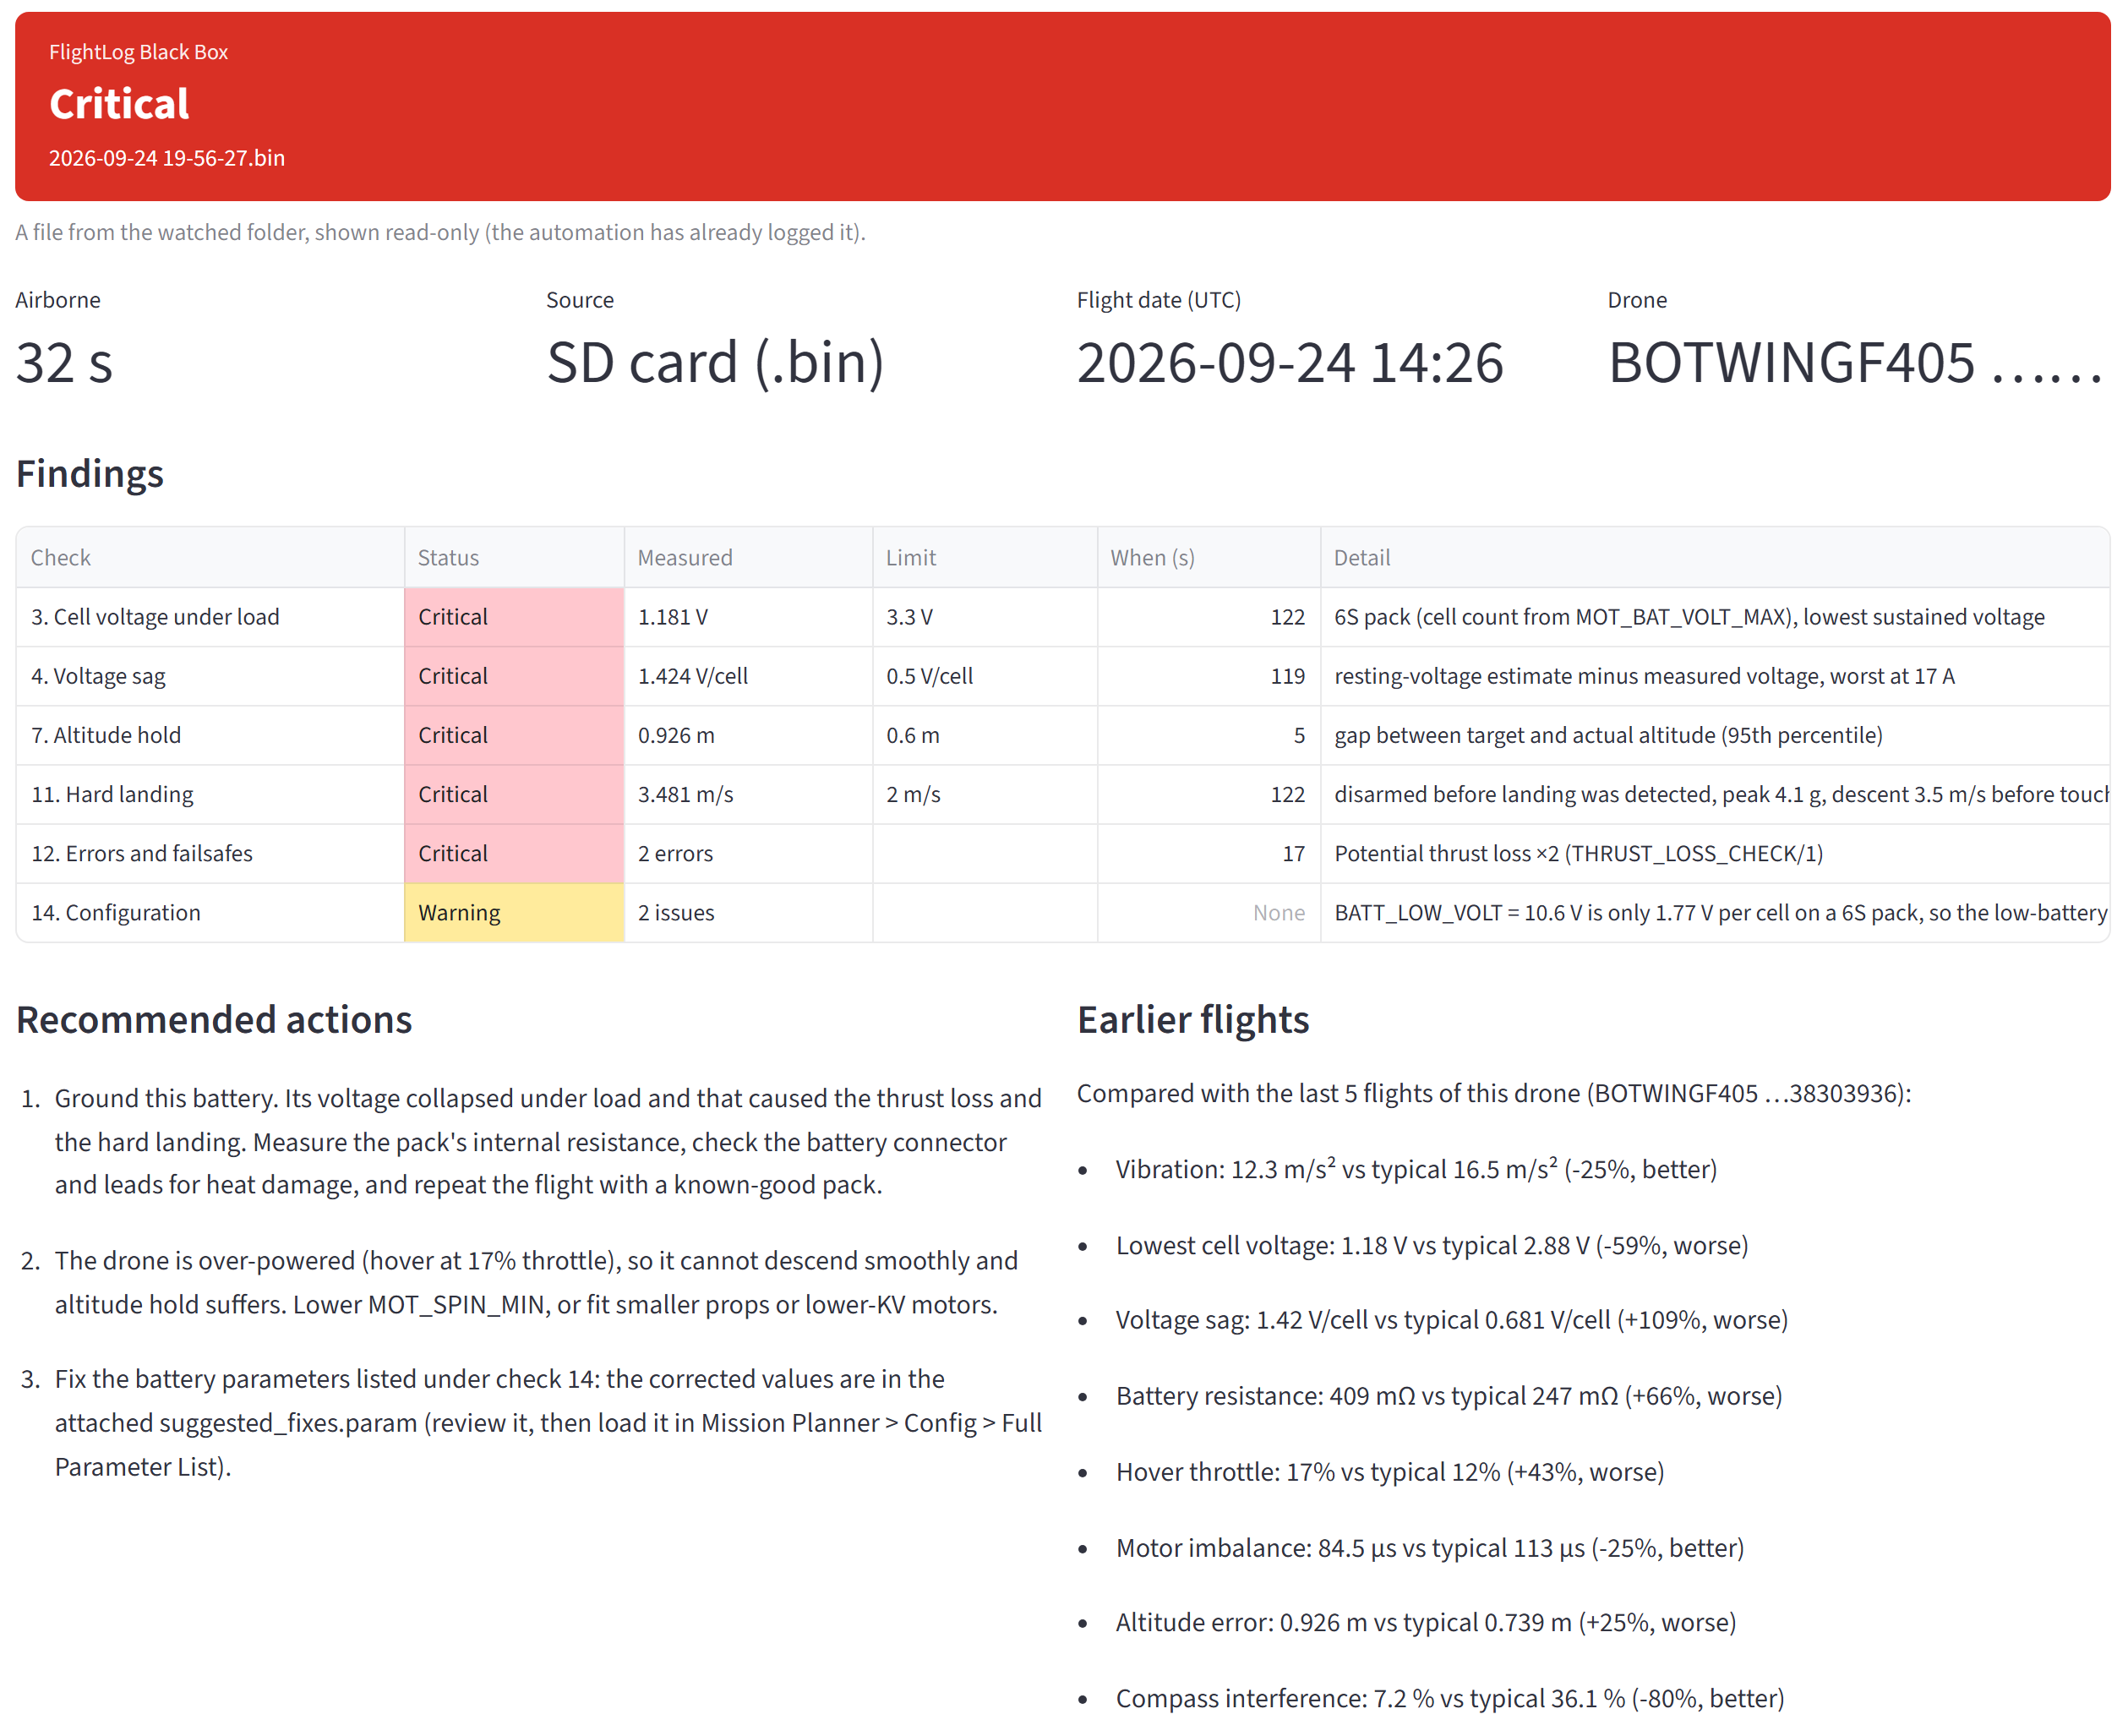
\includegraphics[width=\textwidth]{dashboard_analyse.png}
  \caption{Dashboard, \emph{Analyse a log}, on the 24 September flight.}
  \label{fig:dash}
\end{figure}

\begin{figure}[H]
  \centering
  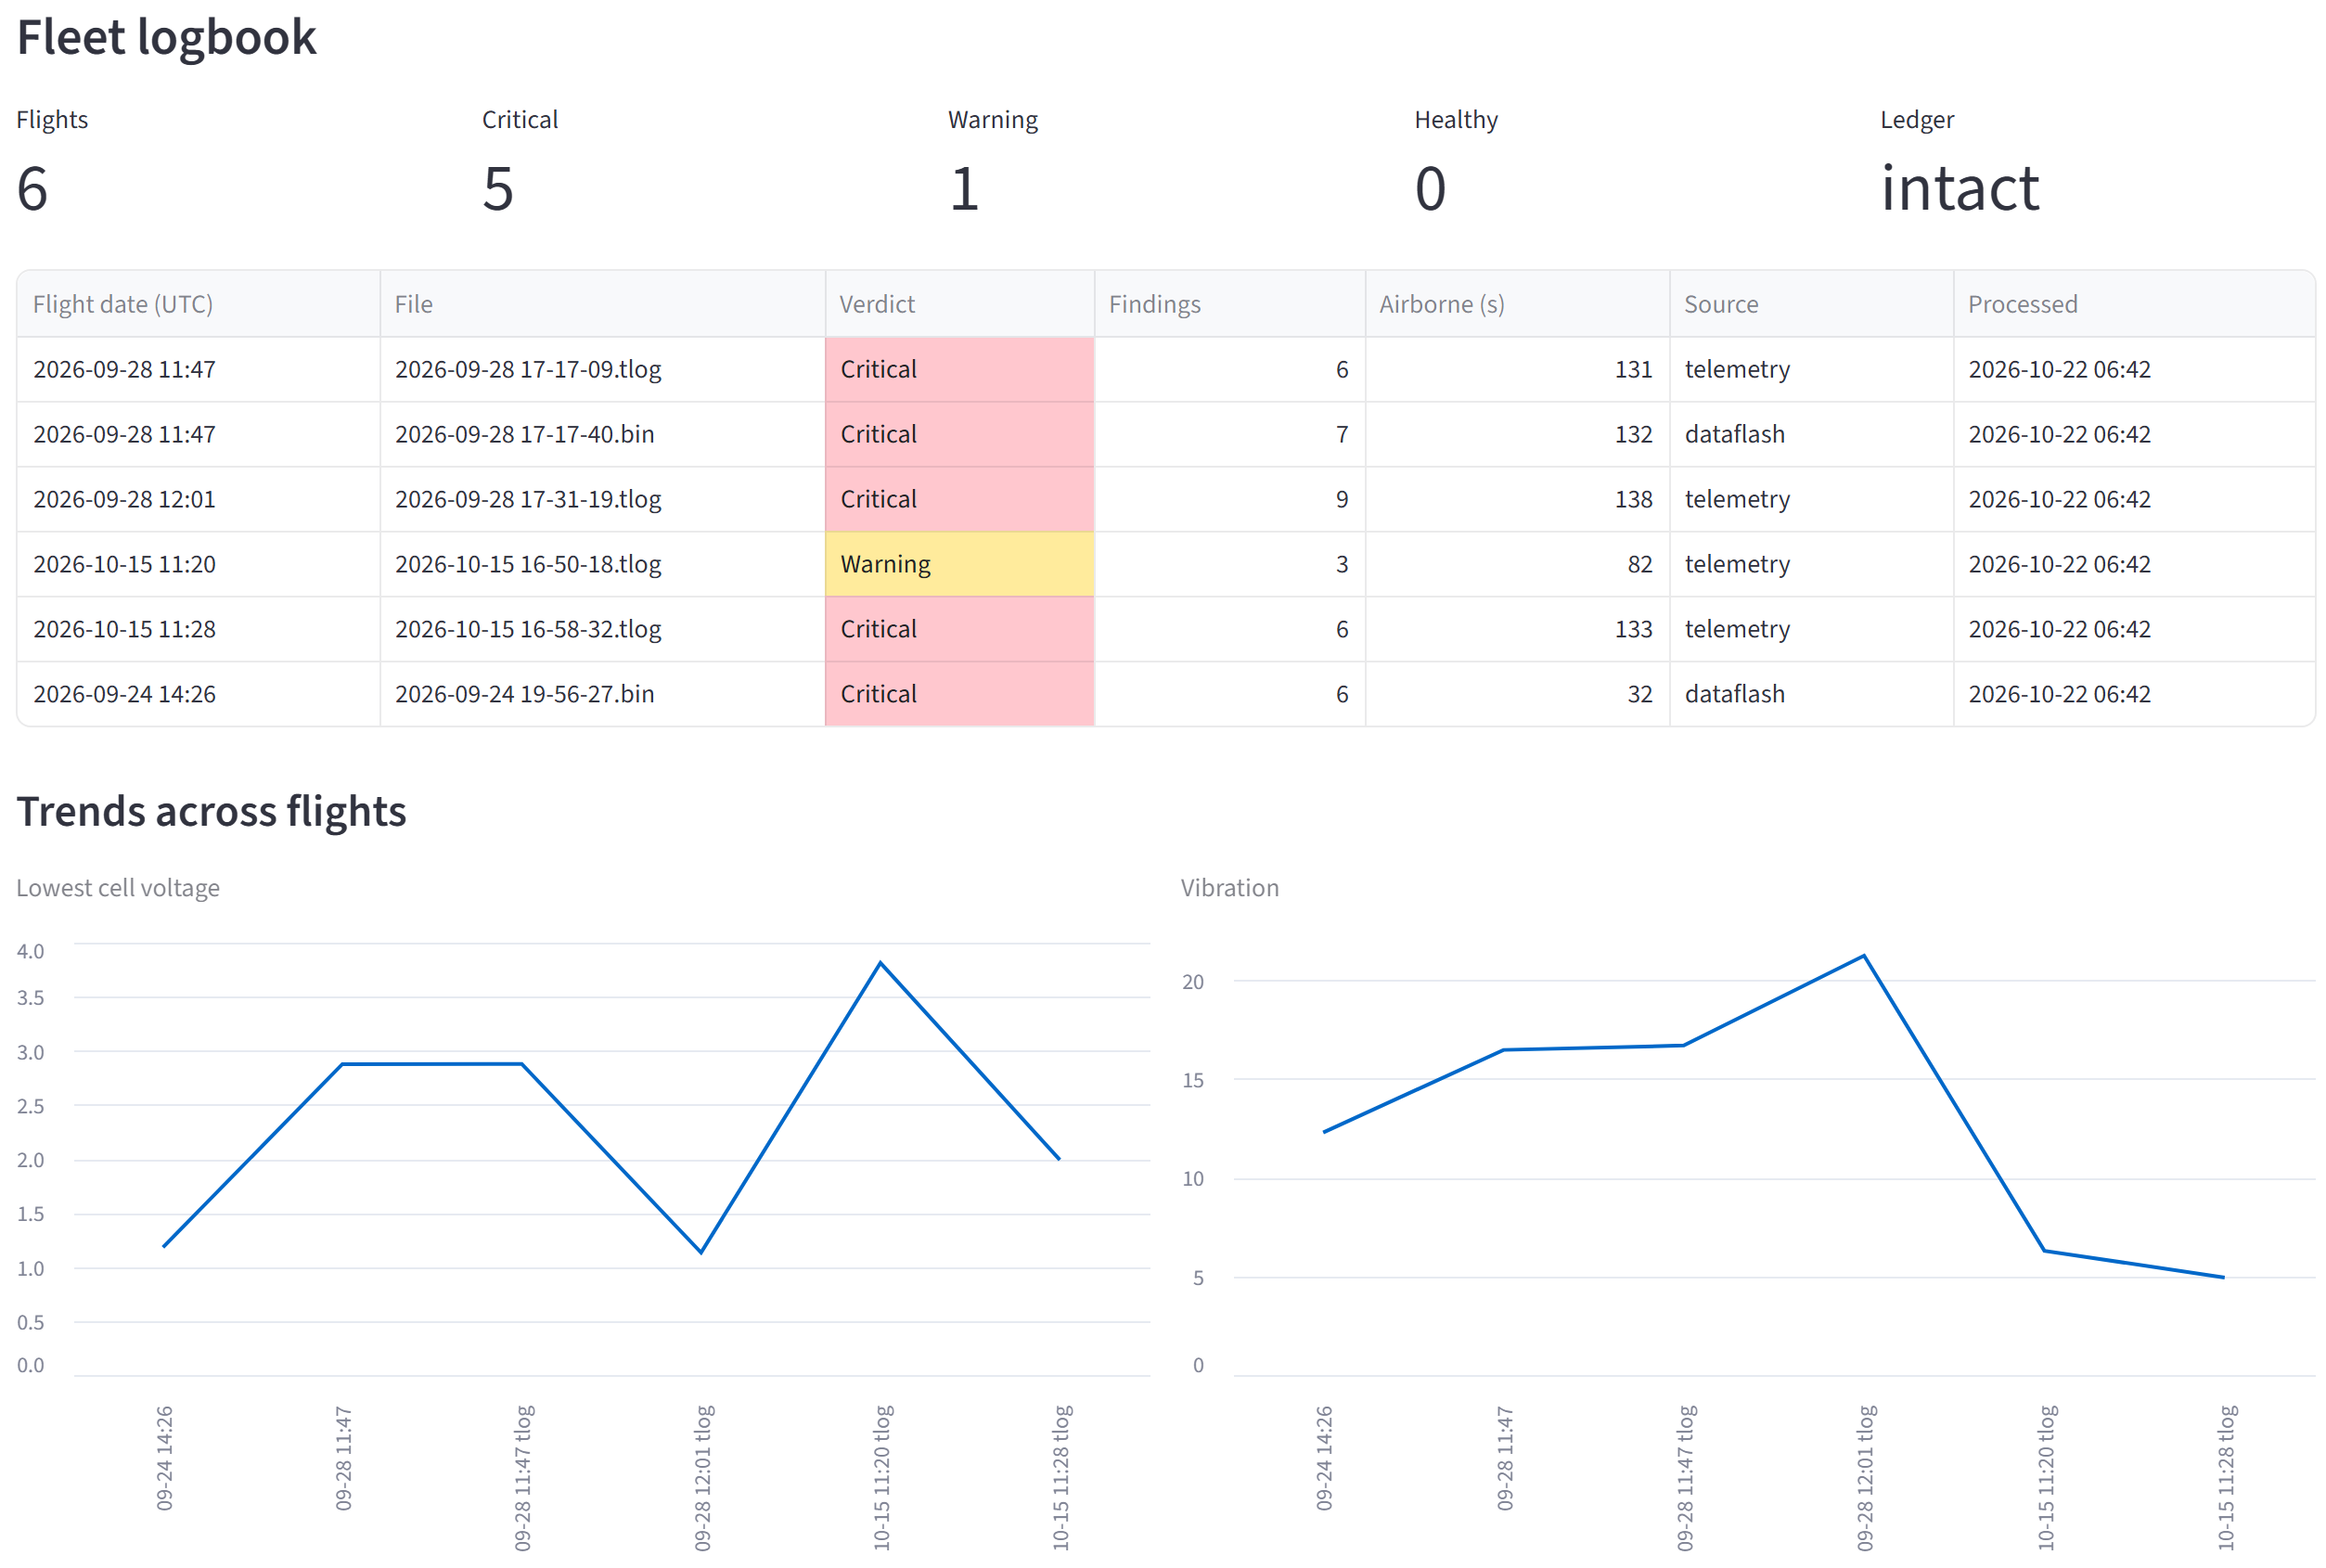
\includegraphics[width=0.85\textwidth]{dashboard_fleet_top.png}
  \caption{Dashboard, \emph{Fleet logbook}, after the six real flight logs.}
  \label{fig:fleet}
\end{figure}

\subsection{n8n automation}
The workflow (Figure~\ref{fig:n8n}) watches the folder with n8n's local file trigger, reads the file, posts it to
the API, turns the base64 attachments into binary items in a Code node, and sends the email over SMTP.

\begin{figure}[H]
  \centering
  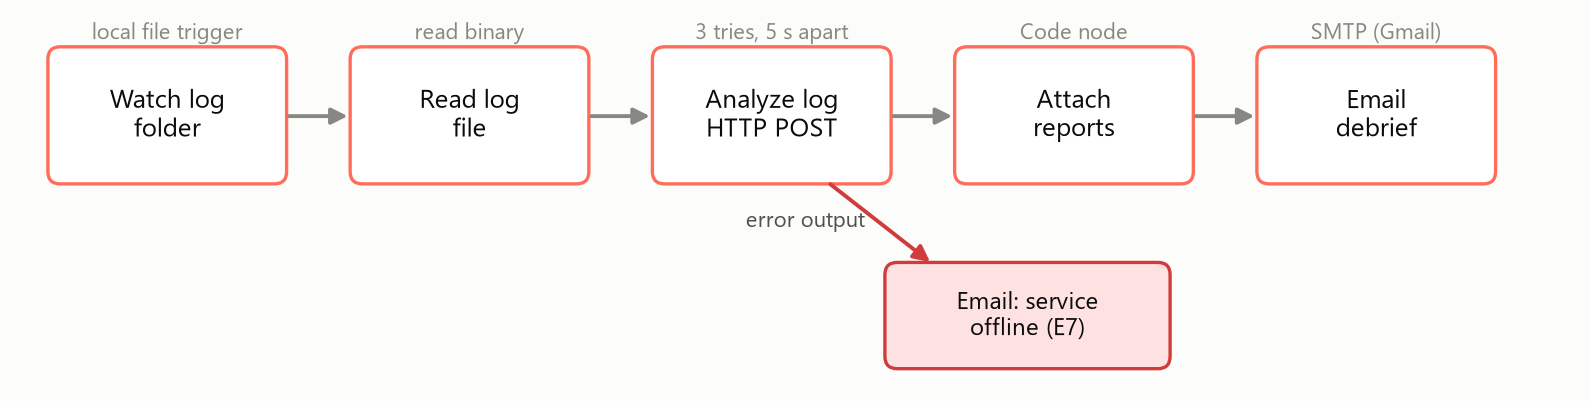
\includegraphics[width=\textwidth]{n8n_workflow.png}
  \caption{The n8n workflow. The HTTP node's error output handles E7.}
  \label{fig:n8n}
\end{figure}

\begin{itemize}
  \item The plan used a Google Drive trigger. Setting up Google OAuth proved too heavy for a lab project, so the
        workflow watches a local folder and sends mail through Gmail SMTP with an App Password.
  \item The folder watcher uses polling and waits for writes to finish, because Windows Explorer locks a file while
        copying it (\code{EBUSY}).
  \item The API address is \code{127.0.0.1}, not \code{localhost}: Node.js 24 resolves \code{localhost} to the IPv6
        address \code{::1}, where uvicorn was not listening.
  \item n8n 2.x disables the local file trigger by default. It is enabled by excluding only the command-execution
        node, and file access is restricted to the watched folder.
  \item \code{scripts/setup_n8n.py} asks for the App Password with a hidden prompt and stores it inside n8n, which
        encrypts it. It is never written to the repository.
\end{itemize}

% ------------------------------------------------------------------ 6
\section{Exception handling}

The brief asks for two exception cases; seven are handled (Table~\ref{tab:exceptions}), and each is recorded in
the logbook's Exceptions sheet.

\begin{table}[H]
  \centering
  \small
  \begin{tabularx}{\textwidth}{@{}lp{3.4cm}p{4.2cm}L@{}}
    \toprule
    \textbf{ID} & \textbf{Scenario} & \textbf{Detected by} & \textbf{What the system does} \\
    \midrule
    E1 & Not a flight log & first bytes match no log format & Rejected; the email says why (and what to upload instead of an \code{.rlog}) \\
    E2 & Corrupt or truncated log & parser stops early, corrupt bytes, log ends armed & Analysed and marked Incomplete; rejected if under 30 s of flight remains \\
    E3 & Message types missing & a needed table is empty & That check is Not available, with the logging option to enable \\
    E4 & Same file again & SHA-256 already in the ledger & Analysed again with a note; counted once in logbook, history and ledger \\
    E5 & Bench log & never armed & Classed No flight, no verdict \\
    E6 & Logbook open in Excel & \code{PermissionError} on save & 3 tries, 10 s apart, then save \code{flight_logbook_pending.xlsx}; the next save includes everything \\
    E7 & Analysis service down & n8n HTTP request fails & 3 tries 5 s apart, then a ``service offline'' email \\
    \bottomrule
  \end{tabularx}
  \caption{Exception cases.}
  \label{tab:exceptions}
\end{table}

The plan originally skipped duplicates (E4). With only a handful of real logs, the team wanted re-uploads to
produce a full report, so a repeat is now analysed again with a note while still being counted only once.

% ------------------------------------------------------------------ 7
\section{Testing}

\subsection{Automated tests}
Each scenario of the test plan is a pytest case (Table~\ref{tab:tests}). Instead of crashing a drone or setting
up the simulator, a small writer in \code{tests/dflog.py} produces valid DataFlash logs with injected faults:
high vibration, a weak motor, a sagging battery, truncation, bench logs, GPS tracks, compass interference and
vibration at a chosen frequency. A similar writer produces telemetry logs. Real logs placed in \code{tests/data}
are run as well.

\begin{table}[H]
  \centering
  \small
  \begin{tabularx}{\textwidth}{@{}lp{3.3cm}p{4.0cm}L@{}}
    \toprule
    \textbf{ID} & \textbf{Scenario} & \textbf{Expected result} & \textbf{Test} \\
    \midrule
    T1 & Clean flight & Healthy & \code{test_t1_clean_flight_is_healthy} \\
    T2 & High vibration & Warning or Critical on 1--2 & \code{test_t2_high_vibration}, \code{..._severe_...} \\
    T3 & Low battery and sag & Critical on 3--4 & \code{test_t3_low_battery_and_sag} \\
    T4 & Motor failure, crash & Critical on 10--12 & \code{test_t4_motor_failure_and_crash} \\
    T5 & Truncated log & Incomplete (E2) & \code{test_t5_truncated_log_is_incomplete} \\
    T6 & Not a log & Rejected (E1) & \code{test_t6_not_a_log} \\
    T7 & Duplicate & Note, counted once (E4) & \code{test_t7_duplicate_...}, \code{test_simultaneous_repeats_count_once} \\
    T8 & Bench log & No flight (E5) & \code{test_t8_bench_log_never_armed} \\
    T9 & Logbook open & Pending copy (E6) & \code{test_e6_logbook_open_in_excel} \\
    T10 & Service down & Offline email (E7) & \code{test_workflow_is_wired_and_has_the_fixes}, and a manual run with the API stopped \\
    \bottomrule
  \end{tabularx}
  \caption{Test plan and the tests that cover it. All pass.}
  \label{tab:tests}
\end{table}

Beyond the plan, tests cover the telemetry parser, \code{.rlog} rejection, each new check, the email wording,
the recommended actions, the KML and \code{.param} exports, history comparison, the pre-flight check, the ledger
detecting an edited entry, path tricks on the download endpoint, the n8n Code node (run in Node.js on a real API
reply) and the dashboard (Streamlit's AppTest). The suite has 88 tests: 83 pass on synthetic logs, and 5 more run
when real logs are placed in \code{tests/data}.

The workflow was also run end to end on a separate n8n instance with a local mail server: \code{.bin},
\code{.tlog} and \code{.rlog} drops, a file still locked while being copied, and the API stopped (E7).

\subsection{Results on the real logs}
All 28 real files were processed: 3 \code{.bin} (two distinct flights and a copy), 13 \code{.tlog} and 12
\code{.rlog}. Six flight logs were analysed (five distinct flights: the 28 September 17:17 flight was recorded both
on the SD card and by the ground station), nine telemetry logs were ground sessions that never armed (E5), and the
\code{.rlog} files were rejected with a message pointing to the matching \code{.tlog}. Figure~\ref{fig:matrix} shows
every check on every flight log. Five are Critical and one is Warning, mainly because of the battery.
Telemetry logs show more ``Not available'' results because they carry less data. Analysing one log takes under
a second.

\begin{figure}[H]
  \centering
  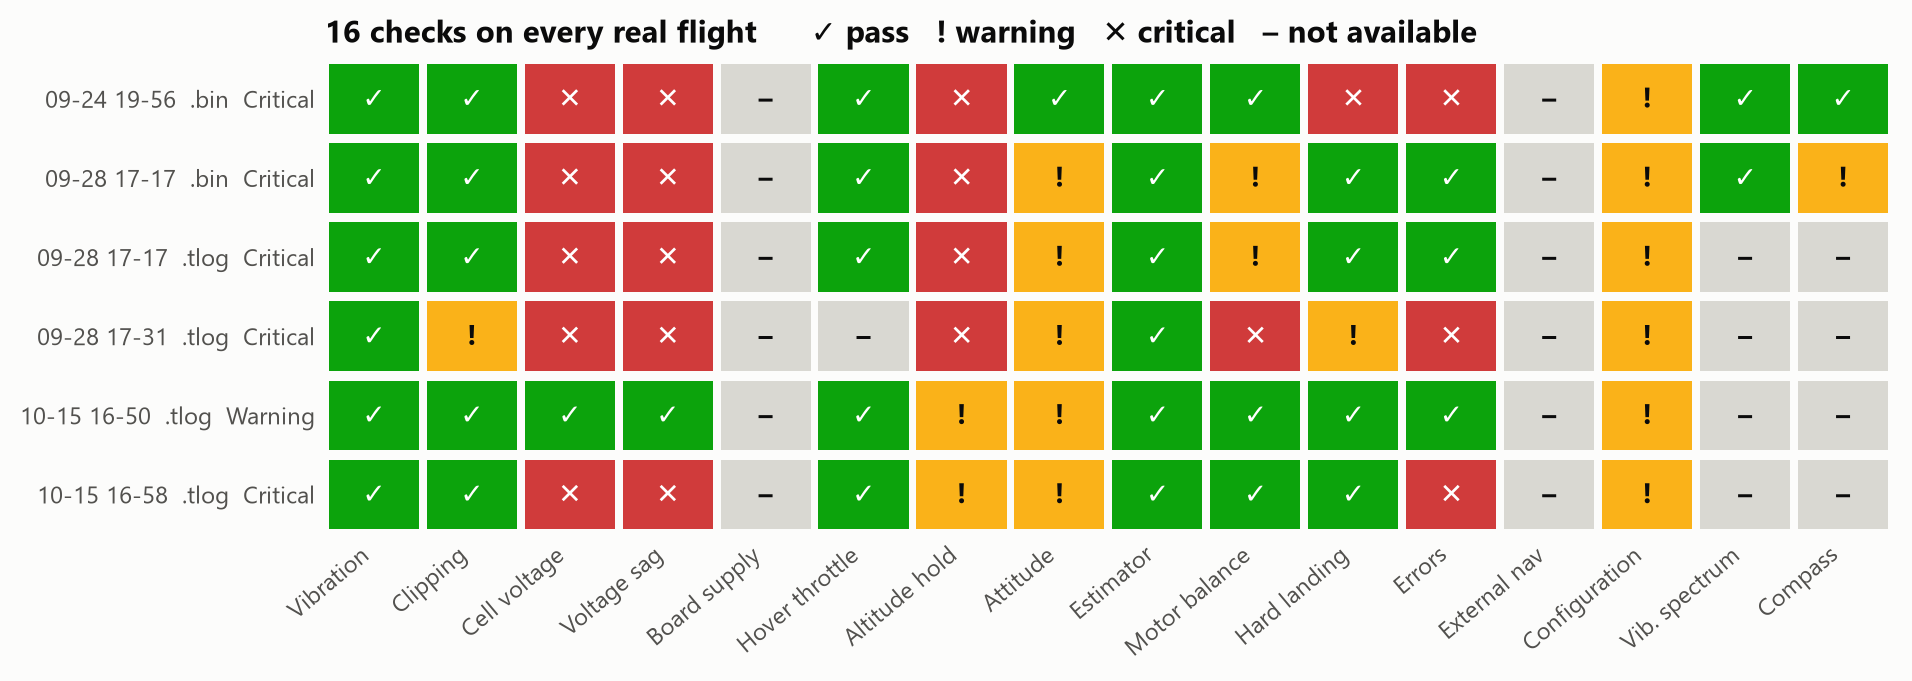
\includegraphics[width=\textwidth]{results_matrix.png}
  \caption{All 16 checks on the six real flight logs.}
  \label{fig:matrix}
\end{figure}

\subsection{Case study: the 24 September flight}
The log holds two short flights. In both, the voltage fell from about 3.6~V to about 1.2~V per cell under
15--18~A, all four motors were driven towards full output, and the flight controller logged ``potential thrust
loss'' (Figures~\ref{fig:crash} and~\ref{fig:motors}). The low-battery failsafe was set to
\code{BATT_LOW_VOLT} = 10.6~V on a 6S pack, only 1.77~V per cell, and \code{BATT_FS_LOW_ACT} = 0, so no failsafe
could ever have acted. The system reports Critical on cell voltage, sag, hard landing and errors, links them into
one action (ground the battery), flags the parameters under check 14 and writes corrected values to
\code{suggested_fixes.param}. Run on the same parameters before the flight, the pre-flight check returns NO-GO.

\begin{figure}[H]
  \centering
  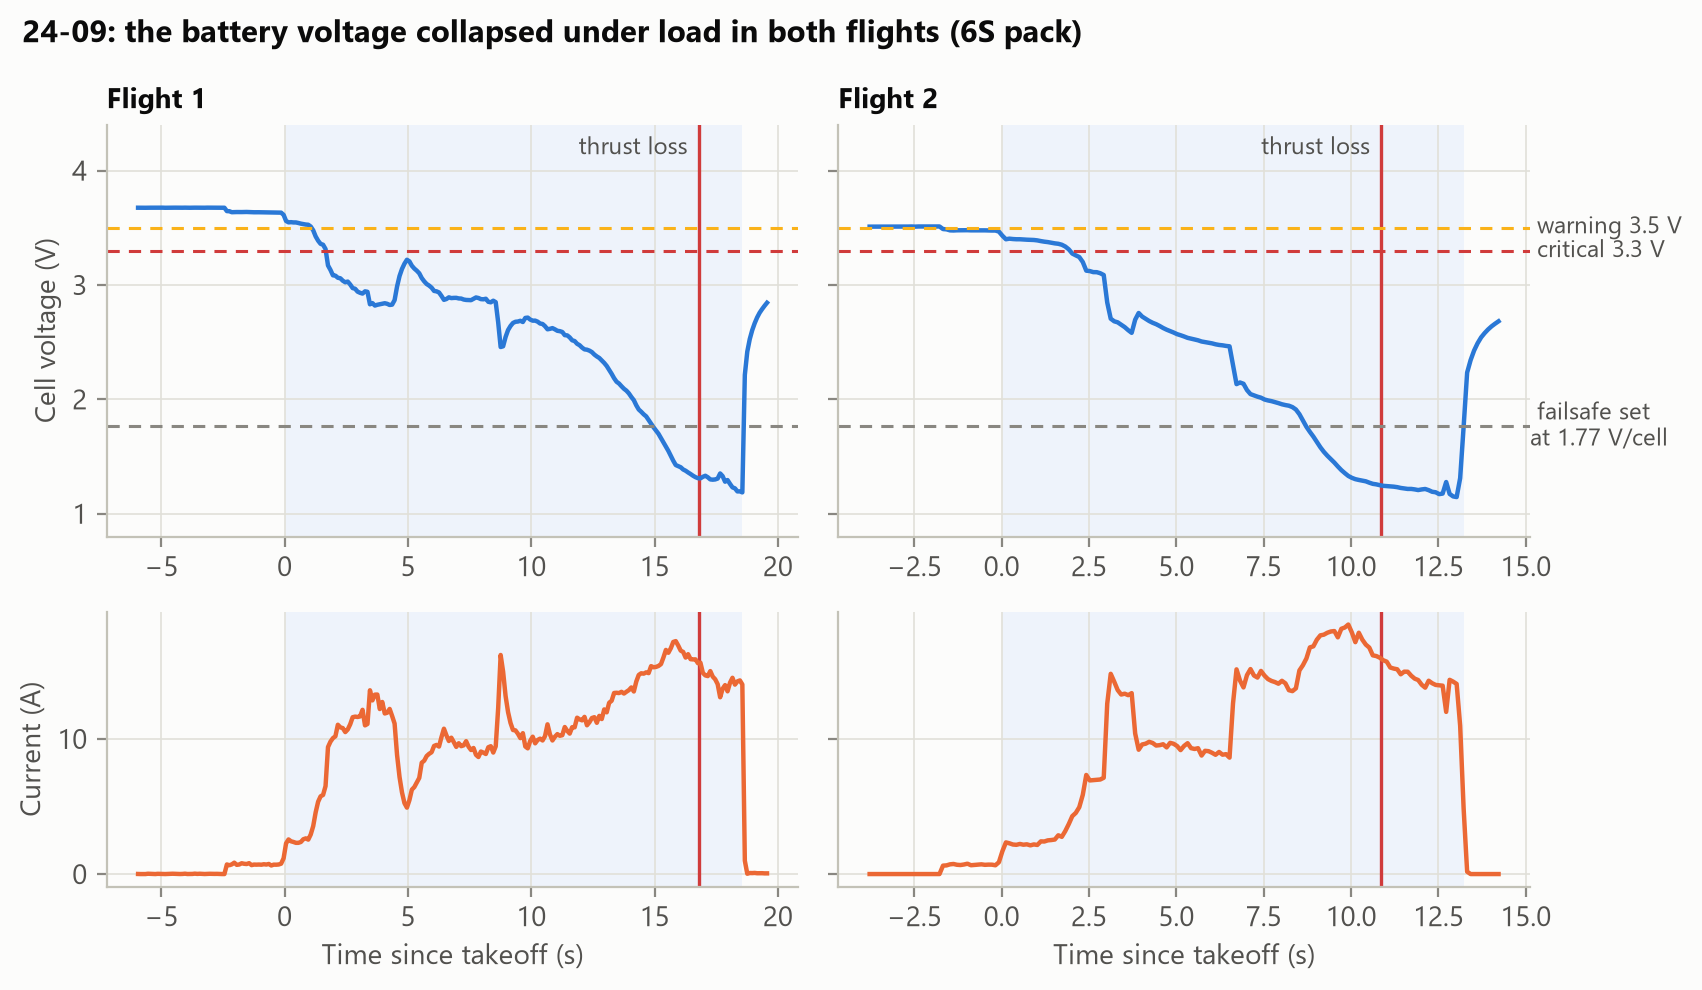
\includegraphics[width=\textwidth]{crash_battery.png}
  \caption{Cell voltage and current in the two 24 September flights. Red lines: the thrust-loss errors.}
  \label{fig:crash}
\end{figure}

\begin{figure}[H]
  \centering
  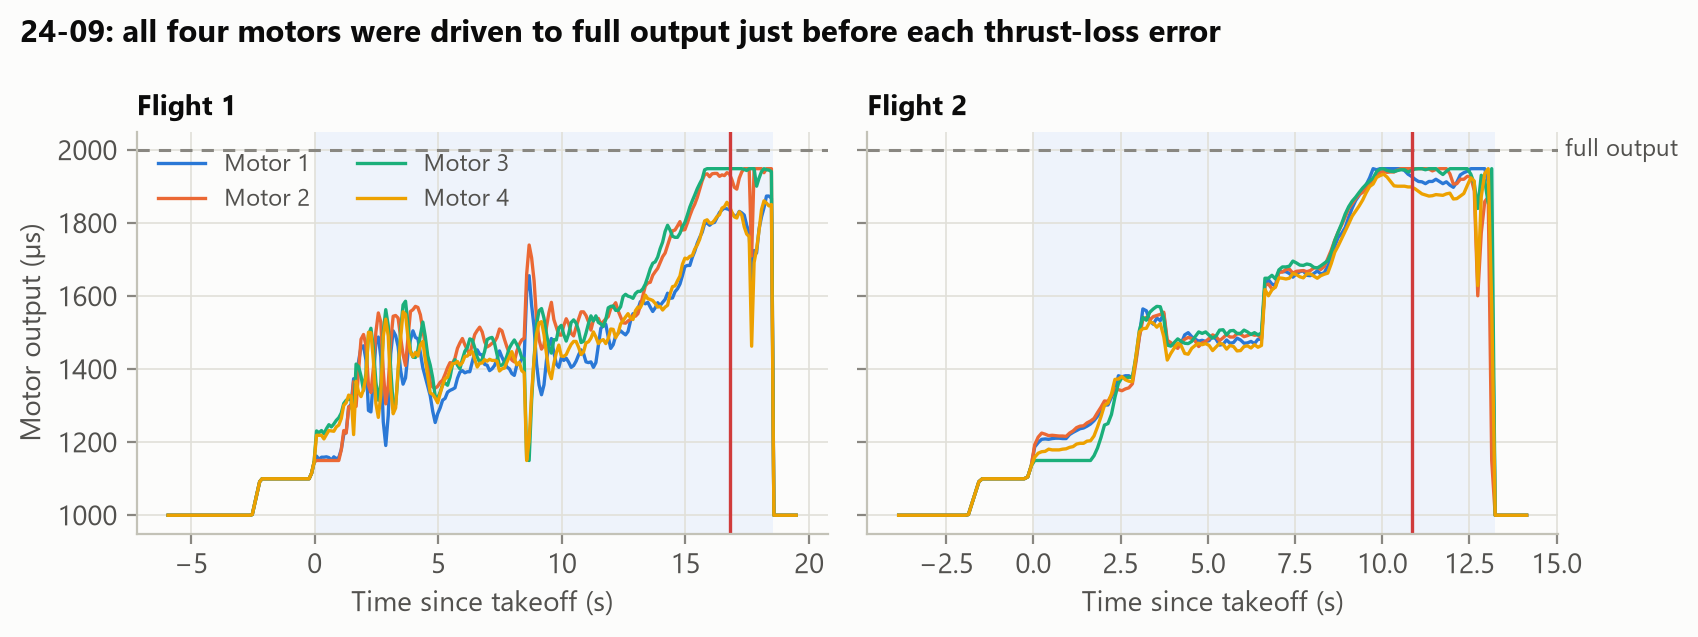
\includegraphics[width=\textwidth]{crash_motors.png}
  \caption{Motor outputs in the same flights.}
  \label{fig:motors}
\end{figure}

\subsection{Checks 15 and 16 on the 28 September flight}
On 28 September the gyro spectrum peaks at 151~Hz (Figure~\ref{fig:spectrum}). The notch filter is set to 80~Hz
with its first two harmonics enabled (\code{INS_HNTCH_HMNCS} = 3) and a 40~Hz bandwidth, so it also acts at
160~Hz, and the peak falls inside that band: check 15 passes. It still notes that throttle tracking is off
(\code{INS_HNTCH_REF} = 0), so the notch stays put while the motor frequency moves with throttle. The compass field rises by about
10~mGauss per amp, 36\% of the Earth's field at full current, above the 30\% limit (Figure~\ref{fig:compass}).

\begin{figure}[H]
  \centering
  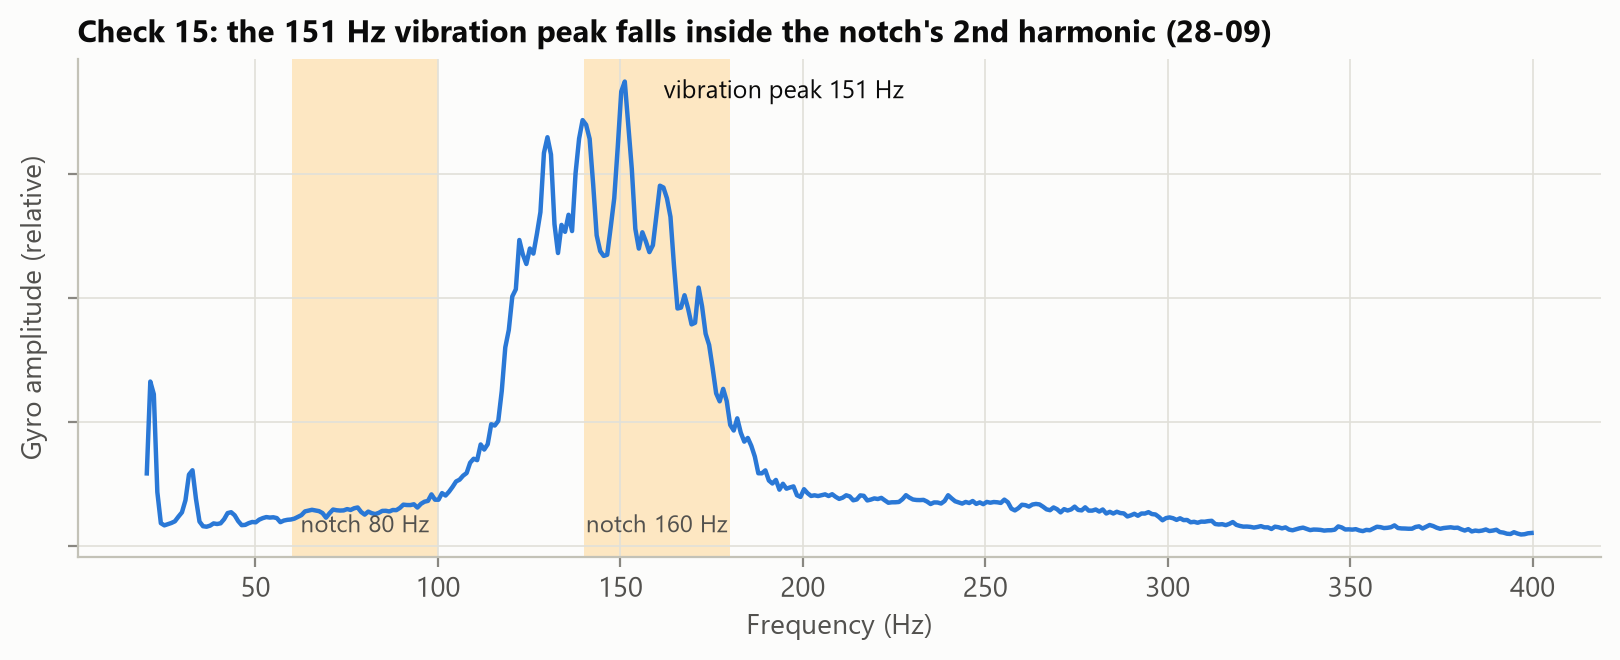
\includegraphics[width=\textwidth]{spectrum.png}
  \caption{Gyro vibration spectrum against the notch filter's two harmonics, 28 September.}
  \label{fig:spectrum}
\end{figure}

\begin{figure}[H]
  \centering
  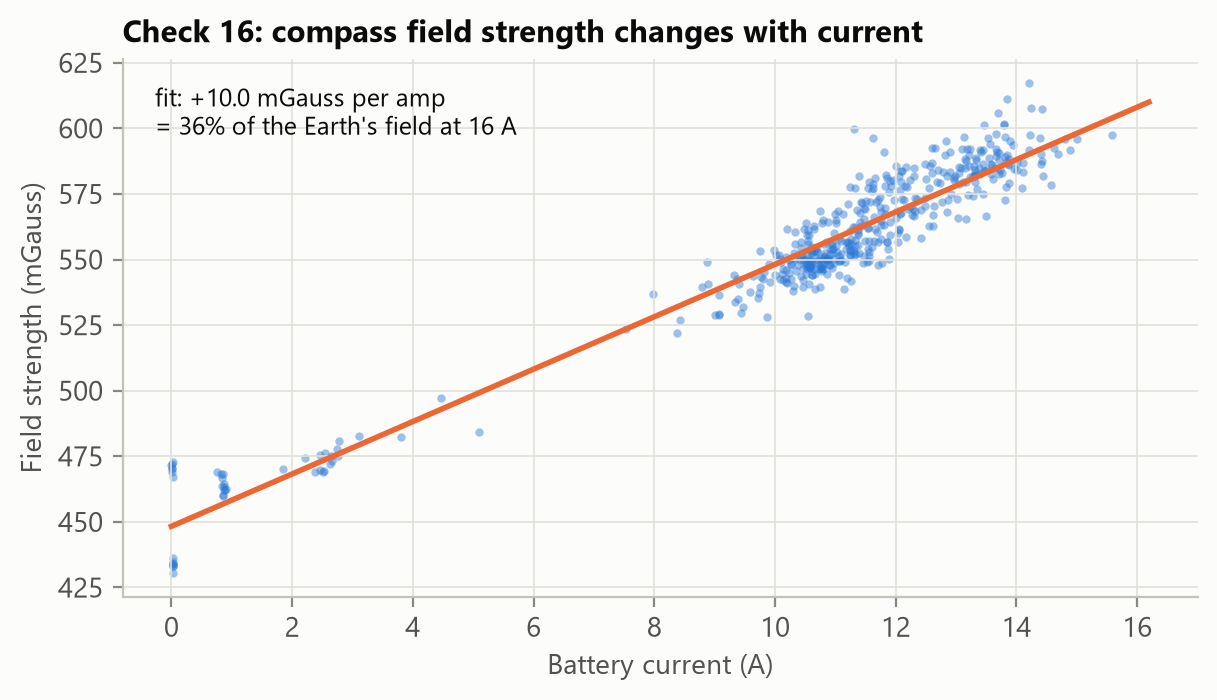
\includegraphics[width=0.72\textwidth]{compass.png}
  \caption{Compass field strength against battery current, 28 September.}
  \label{fig:compass}
\end{figure}

\subsection{Verification against the manual tool}
The reported values can be checked by hand: open the same log in UAV Log Viewer or Mission Planner and plot
\code{BAT.Volt} and \code{VIBE}. For the 24 September log, the lowest sustained cell voltage of 1.18~V corresponds
to about 7.1~V on the 6S pack; the reported values are 1-second rolling medians, so single samples in the viewer
can be slightly lower.
% Add the side-by-side screenshot (UAV Log Viewer next to the report) here before submitting.

% ------------------------------------------------------------------ 8
\section{Discussion}

\paragraph{Changes from the plan.}
The Google Drive trigger became a watched folder with Gmail SMTP; four checks were added (13--16); telemetry logs
are supported with reduced detail; repeat uploads are analysed again instead of skipped; and a pre-flight check,
flight map, parameter fixes, history comparison and ledger were added. The per-flight PowerPoint debrief was
deferred, because the email and dashboard already present the same content.

\paragraph{What the real logs taught us.}
The plan assumed a single airframe and clean logs. The real logs came from a different quadcopter and had a 6S
setting on a 3S pack, aborted arms, bench time with a 0~V battery and radio failsafes, errors logged after
disarming, and Windows file locks. Testing on them early drove the main design decisions: flight windowing,
cell count from the voltage at arming, and file detection by content.

% ------------------------------------------------------------------ 9
\section{Limitations and future work}

\textbf{Limitations.}
\begin{itemize}
  \item Only ArduPilot logs are read.
  \item Team-set limits are starting values; they must be tuned on clean flights of each airframe.
  \item Recommendations are rules: they link only the causes the rules describe and do not diagnose everything.
  \item Telemetry logs arrive at 2--4~Hz, so spikes shorter than about a second can be missed and the hard-landing
        check uses descent rate only.
\end{itemize}

\textbf{Future work.}
\begin{itemize}
  \item The per-flight PowerPoint debrief from the plan.
  \item ESC telemetry checks (temperature, RPM, errors) once the logs carry ESC data.
  \item Anomaly detection once the logbook holds enough healthy flights to learn from.
  \item PX4 \code{.ulg} support and limit profiles per airframe.
\end{itemize}

% ------------------------------------------------------------------ 10
\section{Conclusion}
FlightLog Black Box replaces a slow, person-dependent review with an automatic one. A log dropped into a folder
becomes a verdict with reasons, actions and parameter fixes in the team's inbox, and every flight is recorded in a
logbook and a tamper-evident ledger, so problems that build up across flights become visible. On the team's own
logs it found a battery fault and a misconfigured failsafe that together explain the 24 September thrust loss,
and it would have flagged the failsafe as NO-GO before that flight.

% ------------------------------------------------------------------ appendix
\appendix
\section{Running the system}
\begin{lstlisting}
python -m venv .venv
.venv\Scripts\python -m pip install -r requirements.txt
.venv\Scripts\python scripts\setup_n8n.py        # once: Gmail address, recipients, App Password
powershell -ExecutionPolicy Bypass -File scripts\start.ps1
# then drop a .bin, .tlog or .param into flight-logs\ ; dashboard: http://localhost:8501
.venv\Scripts\python -m pytest -q                 # run the tests
.venv\Scripts\python -m blackbox LOG.bin          # command line
\end{lstlisting}

\section*{References}
\begin{enumerate}[label={[\arabic*]}]
  \item ArduPilot, ``Downloading and analyzing data logs'' and ``Onboard log messages'', \url{https://ardupilot.org/copter/docs/common-downloading-and-analyzing-data-logs-in-mission-planner.html}
  \item ArduPilot, ``Measuring vibration'', \url{https://ardupilot.org/copter/docs/common-measuring-vibration.html}
  \item ArduPilot, ``EKF failsafe'', \url{https://ardupilot.org/copter/docs/ekf-inav-failsafe.html}
  \item ArduPilot, ``Harmonic notch filters'', \url{https://ardupilot.org/copter/docs/common-imu-notch-filtering.html}
  \item ArduPilot, ``Compass--motor calibration'', \url{https://ardupilot.org/copter/docs/common-compass-setup-advanced.html}
  \item pymavlink, \url{https://github.com/ArduPilot/pymavlink}
  \item n8n documentation, \url{https://docs.n8n.io}
  \item FastAPI, \url{https://fastapi.tiangolo.com}; Streamlit, \url{https://docs.streamlit.io}
\end{enumerate}

\end{document}
